\documentclass{ximera}

%\usepackage{todonotes}

\newcommand{\todo}{}

\usepackage{esint} % for \oiint
\ifxake%%https://math.meta.stackexchange.com/questions/9973/how-do-you-render-a-closed-surface-double-integral
\renewcommand{\oiint}{{\large\bigcirc}\kern-1.56em\iint}
\fi


\graphicspath{
  {./}
  {ximeraTutorial/}
  {basicPhilosophy/}
  {functionsOfSeveralVariables/}
  {normalVectors/}
  {lagrangeMultipliers/}
  {vectorFields/}
  {greensTheorem/}
  {shapeOfThingsToCome/}
  {dotProducts/}
  {partialDerivativesAndTheGradientVector/}
  {../productAndQuotientRules/exercises/}
  {../normalVectors/exercisesParametricPlots/}
  {../continuityOfFunctionsOfSeveralVariables/exercises/}
  {../partialDerivativesAndTheGradientVector/exercises/}
  {../directionalDerivativeAndChainRule/exercises/}
  {../commonCoordinates/exercisesCylindricalCoordinates/}
  {../commonCoordinates/exercisesSphericalCoordinates/}
  {../greensTheorem/exercisesCurlAndLineIntegrals/}
  {../greensTheorem/exercisesDivergenceAndLineIntegrals/}
  {../shapeOfThingsToCome/exercisesDivergenceTheorem/}
  {../greensTheorem/}
  {../shapeOfThingsToCome/}
  {../separableDifferentialEquations/exercises/}
  {vectorFields/}
}

\newcommand{\mooculus}{\textsf{\textbf{MOOC}\textnormal{\textsf{ULUS}}}}

\usepackage{tkz-euclide}
\usepackage{tikz}
\usepackage{tikz-cd}
\usetikzlibrary{arrows}
\tikzset{>=stealth,commutative diagrams/.cd,
  arrow style=tikz,diagrams={>=stealth}} %% cool arrow head
\tikzset{shorten <>/.style={ shorten >=#1, shorten <=#1 } } %% allows shorter vectors

\usetikzlibrary{backgrounds} %% for boxes around graphs
\usetikzlibrary{shapes,positioning}  %% Clouds and stars
\usetikzlibrary{matrix} %% for matrix
\usepgfplotslibrary{polar} %% for polar plots
\usepgfplotslibrary{fillbetween} %% to shade area between curves in TikZ
%\usetkzobj{all}
\usepackage[makeroom]{cancel} %% for strike outs
%\usepackage{mathtools} %% for pretty underbrace % Breaks Ximera
%\usepackage{multicol}
\usepackage{pgffor} %% required for integral for loops



%% http://tex.stackexchange.com/questions/66490/drawing-a-tikz-arc-specifying-the-center
%% Draws beach ball
\tikzset{pics/carc/.style args={#1:#2:#3}{code={\draw[pic actions] (#1:#3) arc(#1:#2:#3);}}}



\usepackage{array}
\setlength{\extrarowheight}{+.1cm}
\newdimen\digitwidth
\settowidth\digitwidth{9}
\def\divrule#1#2{
\noalign{\moveright#1\digitwidth
\vbox{\hrule width#2\digitwidth}}}




% \newcommand{\RR}{\mathbb R}
% \newcommand{\R}{\mathbb R}
% \newcommand{\N}{\mathbb N}
% \newcommand{\Z}{\mathbb Z}

\newcommand{\sagemath}{\textsf{SageMath}}


%\renewcommand{\d}{\,d\!}
%\renewcommand{\d}{\mathop{}\!d}
%\newcommand{\dd}[2][]{\frac{\d #1}{\d #2}}
%\newcommand{\pp}[2][]{\frac{\partial #1}{\partial #2}}
% \renewcommand{\l}{\ell}
%\newcommand{\ddx}{\frac{d}{\d x}}

% \newcommand{\zeroOverZero}{\ensuremath{\boldsymbol{\tfrac{0}{0}}}}
%\newcommand{\inftyOverInfty}{\ensuremath{\boldsymbol{\tfrac{\infty}{\infty}}}}
%\newcommand{\zeroOverInfty}{\ensuremath{\boldsymbol{\tfrac{0}{\infty}}}}
%\newcommand{\zeroTimesInfty}{\ensuremath{\small\boldsymbol{0\cdot \infty}}}
%\newcommand{\inftyMinusInfty}{\ensuremath{\small\boldsymbol{\infty - \infty}}}
%\newcommand{\oneToInfty}{\ensuremath{\boldsymbol{1^\infty}}}
%\newcommand{\zeroToZero}{\ensuremath{\boldsymbol{0^0}}}
%\newcommand{\inftyToZero}{\ensuremath{\boldsymbol{\infty^0}}}



% \newcommand{\numOverZero}{\ensuremath{\boldsymbol{\tfrac{\#}{0}}}}
% \newcommand{\dfn}{\textbf}
% \newcommand{\unit}{\,\mathrm}
% \newcommand{\unit}{\mathop{}\!\mathrm}
% \newcommand{\eval}[1]{\bigg[ #1 \bigg]}
% \newcommand{\seq}[1]{\left( #1 \right)}
% \renewcommand{\epsilon}{\varepsilon}
% \renewcommand{\phi}{\varphi}


% \renewcommand{\iff}{\Leftrightarrow}

% \DeclareMathOperator{\arccot}{arccot}
% \DeclareMathOperator{\arcsec}{arcsec}
% \DeclareMathOperator{\arccsc}{arccsc}
% \DeclareMathOperator{\si}{Si}
% \DeclareMathOperator{\scal}{scal}
% \DeclareMathOperator{\sign}{sign}


%% \newcommand{\tightoverset}[2]{% for arrow vec
%%   \mathop{#2}\limits^{\vbox to -.5ex{\kern-0.75ex\hbox{$#1$}\vss}}}
% \newcommand{\arrowvec}[1]{{\overset{\rightharpoonup}{#1}}}
% \renewcommand{\vec}[1]{\arrowvec{\mathbf{#1}}}
% \renewcommand{\vec}[1]{{\overset{\boldsymbol{\rightharpoonup}}{\mathbf{#1}}}}

% \newcommand{\point}[1]{\left(#1\right)} %this allows \vector{ to be changed to \vector{ with a quick find and replace
% \newcommand{\pt}[1]{\mathbf{#1}} %this allows \vec{ to be changed to \vec{ with a quick find and replace
% \newcommand{\Lim}[2]{\lim_{\point{#1} \to \point{#2}}} %Bart, I changed this to point since I want to use it.  It runs through both of the exercise and exerciseE files in limits section, which is why it was in each document to start with.

% \DeclareMathOperator{\proj}{\mathbf{proj}}
% \newcommand{\veci}{{\boldsymbol{\hat{\imath}}}}
% \newcommand{\vecj}{{\boldsymbol{\hat{\jmath}}}}
% \newcommand{\veck}{{\boldsymbol{\hat{k}}}}
% \newcommand{\vecl}{\vec{\boldsymbol{\l}}}
% \newcommand{\uvec}[1]{\mathbf{\hat{#1}}}
% \newcommand{\utan}{\mathbf{\hat{t}}}
% \newcommand{\unormal}{\mathbf{\hat{n}}}
% \newcommand{\ubinormal}{\mathbf{\hat{b}}}

% \newcommand{\dotp}{\bullet}
% \newcommand{\cross}{\boldsymbol\times}
% \newcommand{\grad}{\boldsymbol\nabla}
% \newcommand{\divergence}{\grad\dotp}
% \newcommand{\curl}{\grad\cross}
%\DeclareMathOperator{\divergence}{divergence}
%\DeclareMathOperator{\curl}[1]{\grad\cross #1}
% \newcommand{\lto}{\mathop{\longrightarrow\,}\limits}

% \renewcommand{\bar}{\overline}

\colorlet{textColor}{black}
\colorlet{background}{white}
\colorlet{penColor}{blue!50!black} % Color of a curve in a plot
\colorlet{penColor2}{red!50!black}% Color of a curve in a plot
\colorlet{penColor3}{red!50!blue} % Color of a curve in a plot
\colorlet{penColor4}{green!50!black} % Color of a curve in a plot
\colorlet{penColor5}{orange!80!black} % Color of a curve in a plot
\colorlet{penColor6}{yellow!70!black} % Color of a curve in a plot
\colorlet{fill1}{penColor!20} % Color of fill in a plot
\colorlet{fill2}{penColor2!20} % Color of fill in a plot
\colorlet{fillp}{fill1} % Color of positive area
\colorlet{filln}{penColor2!20} % Color of negative area
\colorlet{fill3}{penColor3!20} % Fill
\colorlet{fill4}{penColor4!20} % Fill
\colorlet{fill5}{penColor5!20} % Fill
\colorlet{gridColor}{gray!50} % Color of grid in a plot

\newcommand{\surfaceColor}{violet}
\newcommand{\surfaceColorTwo}{redyellow}
\newcommand{\sliceColor}{greenyellow}




\pgfmathdeclarefunction{gauss}{2}{% gives gaussian
  \pgfmathparse{1/(#2*sqrt(2*pi))*exp(-((x-#1)^2)/(2*#2^2))}%
}


%%%%%%%%%%%%%
%% Vectors
%%%%%%%%%%%%%

%% Simple horiz vectors
\renewcommand{\vector}[1]{\left\langle #1\right\rangle}


%% %% Complex Horiz Vectors with angle brackets
%% \makeatletter
%% \renewcommand{\vector}[2][ , ]{\left\langle%
%%   \def\nextitem{\def\nextitem{#1}}%
%%   \@for \el:=#2\do{\nextitem\el}\right\rangle%
%% }
%% \makeatother

%% %% Vertical Vectors
%% \def\vector#1{\begin{bmatrix}\vecListA#1,,\end{bmatrix}}
%% \def\vecListA#1,{\if,#1,\else #1\cr \expandafter \vecListA \fi}

%%%%%%%%%%%%%
%% End of vectors
%%%%%%%%%%%%%

%\newcommand{\fullwidth}{}
%\newcommand{\normalwidth}{}



%% makes a snazzy t-chart for evaluating functions
%\newenvironment{tchart}{\rowcolors{2}{}{background!90!textColor}\array}{\endarray}

%%This is to help with formatting on future title pages.
\newenvironment{sectionOutcomes}{}{}



%% Flowchart stuff
%\tikzstyle{startstop} = [rectangle, rounded corners, minimum width=3cm, minimum height=1cm,text centered, draw=black]
%\tikzstyle{question} = [rectangle, minimum width=3cm, minimum height=1cm, text centered, draw=black]
%\tikzstyle{decision} = [trapezium, trapezium left angle=70, trapezium right angle=110, minimum width=3cm, minimum height=1cm, text centered, draw=black]
%\tikzstyle{question} = [rectangle, rounded corners, minimum width=3cm, minimum height=1cm,text centered, draw=black]
%\tikzstyle{process} = [rectangle, minimum width=3cm, minimum height=1cm, text centered, draw=black]
%\tikzstyle{decision} = [trapezium, trapezium left angle=70, trapezium right angle=110, minimum width=3cm, minimum height=1cm, text centered, draw=black]


\title{Analyzing}

\begin{document}

\begin{abstract}
describe everything
\end{abstract}
\maketitle







Completely analyze $T(r) = \tan(\sin(\pi r))$ \\




$\blacktriangleright$  \textbf{\textcolor{blue!55!black}{Domain: }}


We know that $-1 \leq \sin(\pi r) \leq 1$ and $[-1,1] \subset \left( -\frac{\pi}{2}, \frac{\pi}{2} \right)$ and $\tan(x)$ is continuous on $\left( -\frac{\pi}{2}, \frac{\pi}{2} \right)$.  Therefore $T(r)$ is defined for all $r$.  




$\blacktriangleright$  \textbf{\textcolor{blue!55!black}{Continuity: }}




Since both $\tan(x)$ and $\sin(x)$ are continuous, $T$ is the composition of two continuous functions. This also tells us that $T(r)$ is a continuous function.















$T(r)$ will be using $[-1,1]$ out of tangent's $\left( -\frac{\pi}{2}, \frac{\pi}{2} \right)$ waveform.



Graph of $y = T(r)$.

\begin{image}
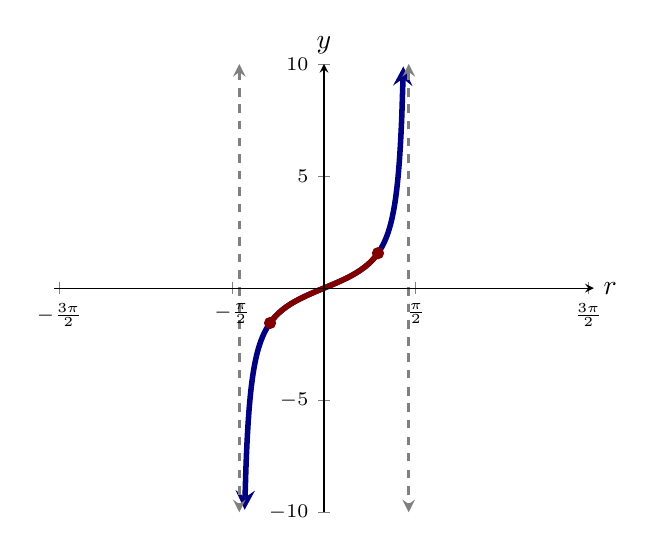
\begin{tikzpicture} 
  \begin{axis}[
            domain=-5:5, ymax=10, xmax=5, ymin=-10, xmin=-5,
            xtick={-4.9, -1.7, 1.7, 4.9}, 
            xticklabels={$-\frac{3\pi}{2}$, $-\frac{\pi}{2}$, $\frac{\pi}{2}$, $\frac{3\pi}{2}$},
            axis lines =center,  xlabel={$r$}, ylabel=$y$,
            ticklabel style={font=\scriptsize},
            every axis y label/.style={at=(current axis.above origin),anchor=south},
            every axis x label/.style={at=(current axis.right of origin),anchor=west},
            axis on top
          ]
          
            \addplot [line width=2, penColor, smooth,samples=100,domain=(-1.47:1.47), <->] {tan(deg(x))};
            \addplot [line width=2, penColor2, smooth,samples=100,domain=(-1:1)] {tan(deg(x))};
            \addplot[color=penColor2,only marks,mark=*] coordinates{(-1,-1.557)}; 
            \addplot[color=penColor2,only marks,mark=*] coordinates{(1,1.557)}; 


      %\addplot[color=penColor,fill=penColor,only marks, mark size=1pt, mark=*] coordinates{(-9,5) (-8,5) (-7,5) (7,5) (8,5) (9,5)};



            \addplot [line width=1, gray, dashed,samples=100,domain=(-10:10), <->] ({-1.57},{x});
            \addplot [line width=1, gray, dashed,samples=100,domain=(-10:10), <->] ({1.57},{x});


           

  \end{axis}
\end{tikzpicture}
\end{image}



$[-1,1]$ is the output of $\sin(\pi r)$, which then becomes the input to tangent.  




For this to happen, the input to sine must be $\left[-\frac{\pi}{2}, \frac{\pi}{2}\right]$, which means that $r \in \left[-\frac{1}{2}, \frac{1}{2}\right]$.


But that is only half the story. \\


As $r$ moves from $-\frac{1}{2}$ to $\frac{1}{2}$, $\sin(\pi r)$ moves from $-1$ to $1$.  As $r$ continues, it moves from $\frac{1}{2}$ to $\frac{3}{2}$ and $\sin(\pi r)$ moves from $1$ back down to $-1$.  Then the whole thing repeats.

Now we have a full period. \\



That gives a full wave over the interval $\left[-\frac{1}{2}, \frac{3}{2}\right]$ and a period of $2$.



As $r$ increases, the sine wave will oscillate between $-1$ and $1$ and this piece of the tangent graph will also oscillate.  






\begin{image}
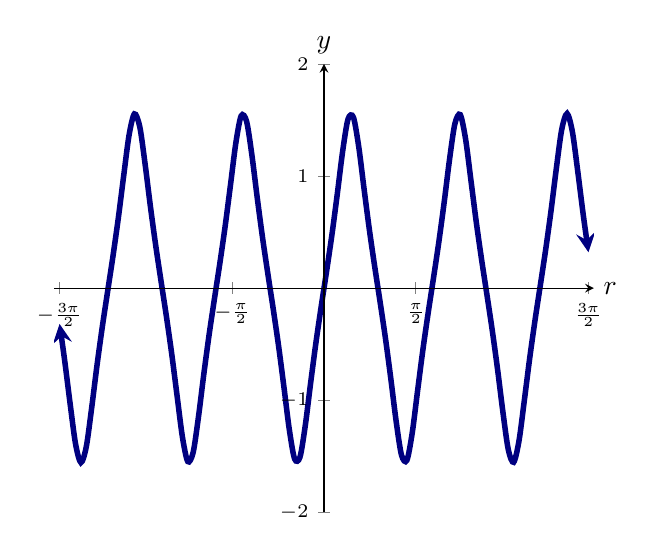
\begin{tikzpicture} 
  \begin{axis}[
            domain=-5:5, ymax=2, xmax=5, ymin=-2, xmin=-5,
            xtick={-4.9, -1.7, 1.7, 4.9}, 
            xticklabels={$-\frac{3\pi}{2}$, $-\frac{\pi}{2}$, $\frac{\pi}{2}$, $\frac{3\pi}{2}$},
            axis lines =center,  xlabel={$r$}, ylabel=$y$,
            ticklabel style={font=\scriptsize},
            every axis y label/.style={at=(current axis.above origin),anchor=south},
            every axis x label/.style={at=(current axis.right of origin),anchor=west},
            axis on top
          ]
          
            \addplot [line width=2, penColor, smooth,samples=100,domain=(-4.9:4.9), <->] {tan(deg(sin(deg(3.1415*x)))};


  \end{axis}
\end{tikzpicture}
\end{image}






Since our period is $\left[-\frac{1}{2}, \frac{3}{2}\right]$, let's regraph with integer tick marks.







\begin{image}
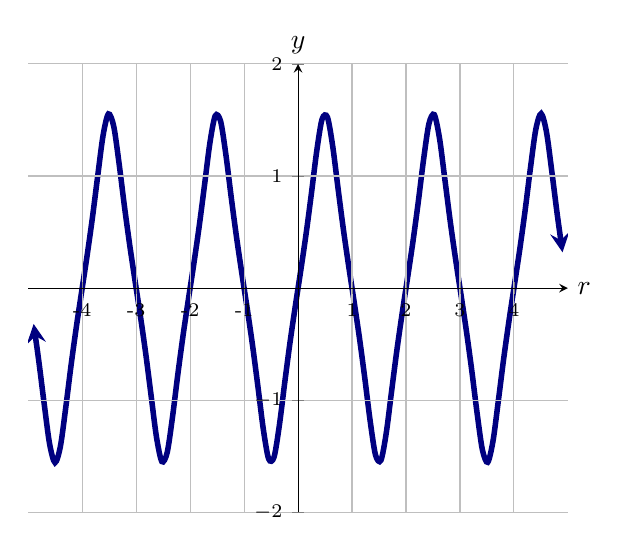
\begin{tikzpicture} 
  \begin{axis}[
            domain=-5:5, ymax=2, xmax=5, ymin=-2, xmin=-5,
            xtick={-4,-3,-2,-1,0,1,2,3,4}, 
            xticklabels={-4,-3,-2,-1,0,1,2,3,4},
            axis lines =center,  xlabel={$r$}, ylabel=$y$, grid = major,
            ticklabel style={font=\scriptsize},
            every axis y label/.style={at=(current axis.above origin),anchor=south},
            every axis x label/.style={at=(current axis.right of origin),anchor=west},
            axis on top
          ]
          
            \addplot [line width=2, penColor, smooth,samples=100,domain=(-4.9:4.9), <->] {tan(deg(sin(deg(3.1415*x)))};


  \end{axis}
\end{tikzpicture}
\end{image}


















$\blacktriangleright$ \textbf{\textcolor{blue!55!black}{Maximums: }}



The maximum of sine is $1$ and it occurs at $\frac{\pi}{2}$.\\

Tangent is an increasing function, so the maximum of $T(r)$ is also going to occur at $\frac{\pi}{2}$. However, in $T(r)$, the inside of sine is $\pi r$.\\


The maximum of the sine waveform occurs at $r = \frac{1}{2}$.


\[   \tan\left(\sin\left(\pi \cdot \frac{1}{2}\right)\right)  =   \tan\left(\sin\left(\frac{\pi}{2}\right)\right)  = \tan(1)  \approx 1.557  \]


The minimum of $-\tan(1) \approx -1.557$ occurs at $r = -\frac{1}{2}$.


That is just for one period. These maximums and minimums are periodic with a period of $2$.







$\blacktriangleright$ \textbf{\textcolor{blue!55!black}{Minimums: }}



The minimum of sine is $-1$ and it occurs at $-\frac{\pi}{2}$.\\

Tangent is an increasing function, so the minimum of $T(r)$ is also going to occur at $-\frac{\pi}{2}$. However, in $T(r)$, the inside of sine is $\pi r$.\\


The minimum of the sine waveform occurs at $r = -\frac{1}{2}$.


\[   \tan\left(\sin\left(-\pi \cdot \frac{1}{2}\right)\right)  =   \tan\left(\sin\left(-\frac{\pi}{2}\right)\right)  = \tan(-1)  \approx -1.557  \]




That is just for one period. These maximums and minimums are periodic with a period of $2$.







We have also discovered that the critical numbers for $T$ are $\left\{ \frac{1}{2} + 2k \, | \, k \in \mathbb{Z} \right\}$ and $\left\{ -\frac{1}{2} + 2k \, | \, k \in \mathbb{Z} \right\}$










$\blacktriangleright$ \textbf{\textcolor{blue!55!black}{Rate-of-Change: }} 


$\tan(t)$ increases on any interval in its domain.  Therefore, $T(r) = \tan(\sin(\pi r))$ will increase and decrease with $\sin(\pi r)$, which we know everything about.




$T(r)$ increases on $\left[ -\frac{1}{2}, \frac{1}{2} \right]$ and decreases on $\left[\frac{1}{2}, \frac{3}{2} \right]$.



And, this agrees with our graph.







\begin{warning} \textbf{\textcolor{red!80!black}{Increasing}}



We have two versions of \textbf{increasing} and we are beginning to notice.



First, we have a Algebra version of increasing.  The Algebra version occurs over an interval.  

$f(x)$ increases on the interval $[a,b]$, provided whenever $c < d$, then $f(c) < f(d)$. \\

We often attach the work \textbf{average} to the Algebra version.\\







Separate from that is a Calculus version of increasing. The Calculus version occurs at a domain number.

$f(x)$ increases at $x=d$, provided $f'(d) > 0$. \\

We often attach the work \textbf{instantaneous} to the Calculus version.\\




These are different.  A function can be increasing at every domain number and yet not be an increasing function over the whole domain.  We'll want to keep these ideas separate.





\end{warning}









\begin{center}
\textbf{\textcolor{green!50!black}{ooooo-=-=-=-ooOoo-=-=-=-ooooo}} \\

more examples can be found by following this link\\ \link[More Examples of Function Analysis]{https://ximera.osu.edu/csccmathematics/precalculus2/precalculus2/functionAnalysis/examples/exampleList}

\end{center}





\end{document}
